\section{中心路径}
\label{sec:lpipm-central-path}

在可行域内部，沿怎样一条路线走，才能既不撞上边界，又最终到达最优解？答案是一条由对偶理论确定的曲线。我们先回顾要用到的对偶事实，再从一维的障碍函数讲起。

\paragraph{标准型与对偶}
本章讨论第~\ref{chap:linear-programming}章的标准型线性规划及其对偶：
\begin{equation}
 \min_{\bm{x}}\ \bm{c}^\top\bm{x}\quad\text{s.t.}\quad\bm{A}\bm{x}=\bm{b},\quad\bm{x}\geq\bm{0},
 \label{eq:lpipm-primal}
\end{equation}
\begin{equation}
 \max_{\bm{y},\bm{s}}\ \bm{b}^\top\bm{y}\quad\text{s.t.}\quad\bm{A}^\top\bm{y}+\bm{s}=\bm{c},\quad\bm{s}\geq\bm{0},
 \label{eq:lpipm-dual}
\end{equation}
其中$\bm{A}\in\mathbb{R}^{m\times n}$满行秩，$\bm{y}\in\mathbb{R}^m$无符号限制，$\bm{s}\in\mathbb{R}^n$称为对偶松弛。两个最优值分别记为$p^\star$和$d^\star$。

那一章的两个结论是本章的出发点。第一个是目标差的恒等式：若$\bm{x}$原始可行，$(\bm{y},\bm{s})$对偶可行，把$\bm{c}=\bm{A}^\top\bm{y}+\bm{s}$和$\bm{b}=\bm{A}\bm{x}$代入目标差，得到
\begin{equation}
 \bm{c}^\top\bm{x}-\bm{b}^\top\bm{y}
 =(\bm{A}^\top\bm{y}+\bm{s})^\top\bm{x}-(\bm{A}\bm{x})^\top\bm{y}
 =\bm{x}^\top\bm{s}.
 \label{eq:lpipm-gap-identity}
\end{equation}
左边称为对偶间隙。因为$\bm{x},\bm{s}\geq\bm{0}$，它非负，这就是弱对偶。

第二个是强对偶：问题可行且最优值有限时，$p^\star=d^\star$。于是$(\bm{x},\bm{y},\bm{s})$最优，当且仅当它同时满足
\begin{equation}
 \bm{A}\bm{x}=\bm{b},\qquad\bm{A}^\top\bm{y}+\bm{s}=\bm{c},\qquad x_is_i=0\ (i=1,\ldots,n),\qquad\bm{x},\bm{s}\geq\bm{0}.
 \label{eq:lpipm-kkt}
\end{equation}
中间的条件是互补松弛。前两组方程是线性的，难处全在$x_is_i=0$：对每个下标，要决定是$x_i$为零还是$s_i$为零。这是一个组合选择，单纯形法用基来做这个选择，一次换基改动一个下标。

全章贯穿下面这个小例子，只有一条等式约束：
\begin{equation}
 \min_{\bm{x}}\ x_1+2x_2+3x_3\quad\text{s.t.}\quad x_1+x_2+x_3=1,\quad\bm{x}\geq\bm{0}.
 \label{eq:lpipm-running}
\end{equation}
这里$n=3$，$m=1$，$\bm{A}=[1\ 1\ 1]$，$b=1$，$\bm{c}=(1,2,3)^\top$。可行集是$\mathbb{R}^3$中以三个单位向量为顶点的三角形。

对偶约束是$y+s_i=c_i$，即$\bm{s}=(1-y,\,2-y,\,3-y)^\top$，$\bm{s}\geq\bm{0}$等价于$y\leq1$，对偶目标就是$y$本身。最优解和最优对偶解都一眼可得：
\[
 \bm{x}^\star=(1,0,0)^\top,\qquad y^\star=1,\qquad\bm{s}^\star=(0,1,2)^\top,\qquad p^\star=d^\star=1.
\]
可以核对$x_i^\star s_i^\star$全为零。

\paragraph{贴边走与穿过去}
图~\ref{fig:lpipm-edge-vs-interior}是第~\ref{chap:simplex-method}章的工厂问题。黄线是单纯形法的路线，它贴着边界，在三个拐角上各做了一次选择。绿线是本节要建立的路径，它从内部一个点出发，平滑地弯向最优顶点，途中不需要决定任何“走哪条边”的问题。

可以把可行域想成一间房间，最优解在墙角。贴墙走，每到拐角都要判断往哪边转；从房间中央穿过去，没有拐角，但需要两样东西：一种不让人撞墙的力，以及一种随时间减弱这个力的办法，否则永远到不了墙角。这个比喻在终点处失效：真正的解就在墙上，所以排斥力必须在极限中消失，下面的$\mu\downarrow0$就是这件事。

\begin{BookInlineFigure}
  \centering
  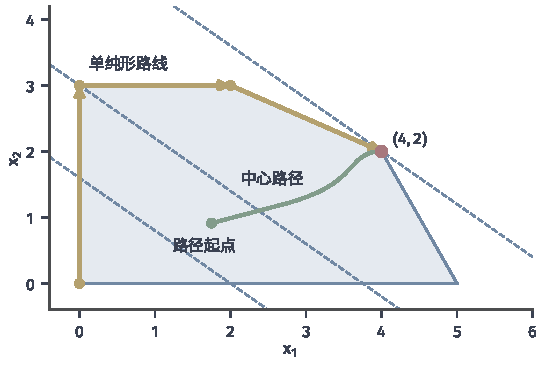
\includegraphics[width=92mm]{figures/05-optimization/01-linear-programming/matplotlib/lpipm-edge-vs-interior/figure.pdf}
  \caption{工厂问题的两条路线。浅蓝区域是可行域，蓝色虚线是利润的等值线，红点是最优顶点$(4,2)$。黄线是单纯形法经过的顶点序列$(0,0)$、$(0,3)$、$(2,3)$、$(4,2)$；绿线是中心路径，从$\mu$很大时的内部点出发，随$\mu$减小弯向最优顶点，全程不碰边界。}
  \label{fig:lpipm-edge-vs-interior}
\end{BookInlineFigure}

\paragraph{一维的障碍}
先看最简单的情形：在$x\geq0$上最小化$f(x)=x$，解是边界点$x=0$。在目标上加一项$-\mu\log x$，其中$\mu>0$，它在$x\downarrow0$时趋于$+\infty$，像一堵逐渐升高的墙，把迭代挡在$x>0$的一侧。这时要解的是
\[
 \min_{x>0}\ x-\mu\log x.
\]
令导数$1-\mu/x$为零，得到唯一的最小点
\[
 x=\mu.
\]
图~\ref{fig:lpipm-log-barrier}显示了两件事。图(a)中，$\mu$越小，墙贴得越紧，离墙稍远的地方几乎不受影响。图(b)中，绿点是加了障碍后的最小点，它随$\mu$减小沿$x=\mu$滑向真正的解$x=0$。

\begin{BookInlineFigure}
  \centering
  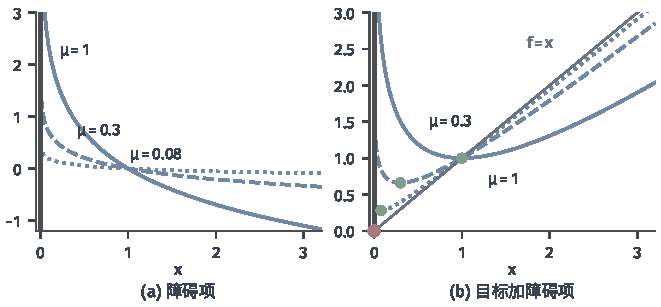
\includegraphics[width=112mm]{figures/05-optimization/01-linear-programming/matplotlib/lpipm-log-barrier/figure.pdf}
  \caption{一维的对数障碍。(a)障碍项$-\mu\log x$，实线、虚线、点线分别对应$\mu=1,0.3,0.08$，深灰粗线是边界$x=0$。(b)目标$f(x)=x$（细灰线）加上障碍项后的三条曲线，绿点是各自的最小点$x=\mu$，红点是真正的解$x=0$。}
  \label{fig:lpipm-log-barrier}
\end{BookInlineFigure}

\paragraph{对数障碍问题}
回到问题~\eqref{eq:lpipm-primal}，对每个坐标都加一项障碍。这里要留意“内部”的含义。例~\eqref{eq:lpipm-running}的可行集是$\mathbb{R}^3$中的一块三角形，厚度为零，没有通常意义下的内点。障碍只负责不等式$\bm{x}\geq\bm{0}$，等式$\bm{A}\bm{x}=\bm{b}$始终严格保持，所以内部是相对等式约束而言的，指满足等式且所有分量为正的点。

\begin{definition}[严格可行]
\label{def:lpipm-strictly-feasible}
满足$\bm{A}\bm{x}=\bm{b}$且$\bm{x}>\bm{0}$的点称为原始\term{严格可行}（strictly feasible）点。满足$\bm{A}^\top\bm{y}+\bm{s}=\bm{c}$且$\bm{s}>\bm{0}$的$(\bm{y},\bm{s})$称为对偶严格可行点。两者都存在时，记
\begin{equation}
 \mathcal{F}^{\circ}=\bigl\{(\bm{x},\bm{y},\bm{s}):\bm{A}\bm{x}=\bm{b},\ \bm{A}^\top\bm{y}+\bm{s}=\bm{c},\ \bm{x}>\bm{0},\ \bm{s}>\bm{0}\bigr\}.
 \label{eq:lpipm-strict-set}
\end{equation}
\end{definition}

严格可行点不一定存在。约束$x_1+x_2=0$、$\bm{x}\geq\bm{0}$的可行集只有原点，其中没有正的点。例~\eqref{eq:lpipm-running}中，$\bm{x}=(1/3,1/3,1/3)^\top$与$y=0$、$\bm{s}=(1,2,3)^\top$都严格可行。

对$\mu>0$，定义\term{对数障碍}（logarithmic barrier）问题
\begin{equation}
 \min_{\bm{x}}\ B_\mu(\bm{x})=\bm{c}^\top\bm{x}-\mu\sum_{i=1}^n\log x_i
 \quad\text{s.t.}\quad\bm{A}\bm{x}=\bm{b},\quad\bm{x}>\bm{0}.
 \label{eq:lpipm-barrier}
\end{equation}
图~\ref{fig:lpipm-bowls}画出例~\eqref{eq:lpipm-running}中$B_\mu$的等值线。线性目标本身没有碗底，障碍项在三条边上竖起墙，围出一个碗。$\mu$大时碗底靠近三角形中央，$\mu$小时墙贴向边界，碗底被线性目标推向最优顶点。

\begin{BookInlineFigure}
  \centering
  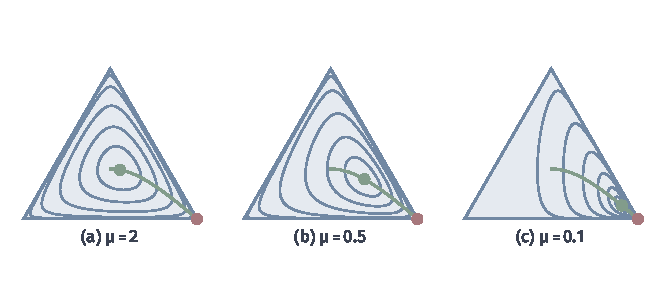
\includegraphics[width=112mm]{figures/05-optimization/01-linear-programming/matplotlib/lpipm-bowls/figure.pdf}
  \caption{例~\eqref{eq:lpipm-running}的障碍目标$B_\mu$在三角形上的等值线（蓝线）。绿线是全部碗底连成的曲线，绿点是当前$\mu$的碗底，红点是最优顶点。$\mu$减小时，碗底沿绿线向红点移动，碗也越来越贴近边界。}
  \label{fig:lpipm-bowls}
\end{BookInlineFigure}

\paragraph{一阶条件给出扰动的互补}
$B_\mu$的梯度是$\bm{c}-\mu\bm{X}^{-1}\bm{1}$，其中$\bm{X}=\operatorname{diag}(\bm{x})$，$\bm{1}$是全一向量。在仿射集合$\{\bm{x}:\bm{A}\bm{x}=\bm{b}\}$上，能移动的方向是$\bm{A}$的零空间，一阶条件要求梯度与零空间正交。$\bm{A}$的零空间的正交补是$\bm{A}^\top$的列空间，所以一阶条件是：存在$\bm{y}$使
\[
 \bm{c}-\mu\bm{X}^{-1}\bm{1}=\bm{A}^\top\bm{y}.
\]

这里出现了一个与$\bm{c}-\bm{A}^\top\bm{y}$相等的正向量，正是对偶松弛的样子。令$\bm{s}=\mu\bm{X}^{-1}\bm{1}$，上式成为$\bm{A}^\top\bm{y}+\bm{s}=\bm{c}$，而$\bm{s}$的定义就是$x_is_i=\mu$。三组条件合起来是
\begin{equation}
 \bm{A}\bm{x}=\bm{b},\qquad\bm{A}^\top\bm{y}+\bm{s}=\bm{c},\qquad x_is_i=\mu\ (i=1,\ldots,n),\qquad\bm{x},\bm{s}>\bm{0}.
 \label{eq:lpipm-central}
\end{equation}
把它与最优性条件~\eqref{eq:lpipm-kkt}逐项对比，只有互补松弛一处不同：$x_is_i=0$换成了$x_is_i=\mu$。

图~\ref{fig:lpipm-complementarity-corner}说明这个改动的好处。在$(x_i,s_i)$平面上，$x_is_i=0$、$x_i,s_i\geq0$是一个直角折线，组合选择就是选落在哪条腿上。把它换成双曲线$x_is_i=\mu$，折角被磨圆了，曲线是光滑的，可以用微积分处理；$\mu$越小，曲线越贴近折角。

\begin{BookInlineFigure}
  \centering
  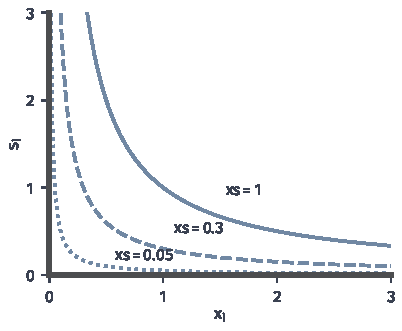
\includegraphics[width=68mm]{figures/05-optimization/01-linear-programming/matplotlib/lpipm-complementarity-corner/figure.pdf}
  \caption{互补条件的光滑化。深灰粗线是$x_is_i=0$、$x_i,s_i\geq0$的直角折线，蓝色曲线是$x_is_i=\mu$，实线、虚线、点线分别对应$\mu=1,0.3,0.05$。$\mu\downarrow0$时曲线贴近折线，但对每个正的$\mu$，$x_i$和$s_i$都严格为正。}
  \label{fig:lpipm-complementarity-corner}
\end{BookInlineFigure}

\paragraph{存在唯一的条件}
碗底并不总是存在，下面的定理说明它需要原始和对偶两侧都有严格可行点。

\begin{theorem}[中心点的存在唯一]
\label{thm:lpipm-central-exists}
设$\bm{A}$满行秩，$\mu>0$。方程组~\eqref{eq:lpipm-central}有解，当且仅当$\mathcal{F}^{\circ}$非空。此时解$(\bm{x}(\mu),\bm{y}(\mu),\bm{s}(\mu))$唯一，且$\bm{x}(\mu)$是障碍问题~\eqref{eq:lpipm-barrier}的唯一最小点。
\end{theorem}

\begin{proof}
必要性：方程组的解本身就是$\mathcal{F}^{\circ}$中的点。

充分性分两步。先证最小点存在。取$(\bar{\bm{y}},\bar{\bm{s}})$对偶严格可行，在原始可行点上，由$\bm{c}=\bm{A}^\top\bar{\bm{y}}+\bar{\bm{s}}$和$\bm{A}\bm{x}=\bm{b}$，目标可以改写为
\[
 \bm{c}^\top\bm{x}=\bm{b}^\top\bar{\bm{y}}+\bar{\bm{s}}^\top\bm{x},
\]
于是
\[
 B_\mu(\bm{x})=\bm{b}^\top\bar{\bm{y}}+\sum_{i=1}^n\bigl(\bar{s}_ix_i-\mu\log x_i\bigr).
\]
因为$\bar{s}_i>0$，每个一元函数$\bar{s}_it-\mu\log t$在$(0,\infty)$上有下界，并且在$t\downarrow0$和$t\to\infty$时都趋于$+\infty$。

于是对原始严格可行点$\bm{x}^{(0)}$，考虑下水平集
\[
 \bigl\{\bm{x}:\bm{A}\bm{x}=\bm{b},\ \bm{x}>\bm{0},\ B_\mu(\bm{x})\leq B_\mu(\bm{x}^{(0)})\bigr\}.
\]
其中每个坐标都落在某个区间$[\epsilon,R]$内，$\epsilon>0$，这是非空紧集。连续函数在紧集上取到最小值，这就是障碍问题的一个最小点。

再证一阶条件与最小点等价，并得到唯一性。最小点在相对内部，一阶条件成立，于是得到方程组~\eqref{eq:lpipm-central}的一个解。反过来，设$(\bm{x},\bm{y},\bm{s})$是一个解。函数$-\log t$是凸函数，所以$B_\mu$在可行集上是严格凸的，对任何可行的$\bm{x}'$有
\[
 B_\mu(\bm{x}')\geq B_\mu(\bm{x})+\nabla B_\mu(\bm{x})^\top(\bm{x}'-\bm{x})=B_\mu(\bm{x})+\bm{y}^\top\bm{A}(\bm{x}'-\bm{x})=B_\mu(\bm{x}),
\]
这说明$\bm{x}$是最小点。严格凸性保证最小点唯一，于是$\bm{x}$唯一，$\bm{s}=\mu\bm{X}^{-1}\bm{1}$也唯一。$\bm{A}^\top$列满秩，$\bm{A}^\top\bm{y}=\bm{c}-\bm{s}$给出唯一的$\bm{y}$。
\end{proof}

对偶严格可行这个条件不能省。问题$\min 0$、$x_1-x_2=0$、$\bm{x}\geq\bm{0}$有原始严格可行点$(1,1)$，最优值为$0$。它的障碍目标在可行射线$x_1=x_2=r$上等于$-2\mu\log r$，当$r\to\infty$时趋于$-\infty$，没有最小点。原因在对偶一侧：对偶约束$y+s_1=0$、$-y+s_2=0$迫使$s_1+s_2=0$，严格可行点不存在。

\begin{definition}[中心路径]
\label{def:lpipm-central-path}
当$\mathcal{F}^{\circ}$非空时，$\mu$取遍$(0,\infty)$，方程组~\eqref{eq:lpipm-central}的解构成一条曲线
\begin{equation}
 \mathcal{C}=\bigl\{(\bm{x}(\mu),\bm{y}(\mu),\bm{s}(\mu)):\mu>0\bigr\},
 \label{eq:lpipm-central-path}
\end{equation}
称为\term{中心路径}（central path）。其中的点称为中心点。
\end{definition}

这个名字可以这样理解：方程组要求所有乘积$x_is_i$相等，没有哪个坐标比别的坐标更靠近自己的边界，点保持在“中央”。下面的例子把路径完整地写出来。

\begin{example}[贯穿例的中心路径]
\label{ex:lpipm-central-closed-form}
在问题~\eqref{eq:lpipm-running}中，$s_i=c_i-y$，$x_is_i=\mu$给出$x_i=\mu/(c_i-y)$。代入$x_1+x_2+x_3=1$，消去$\bm{x}$，得到$\mu$与$y$的关系
\[
 \mu=\Bigl(\frac{1}{1-y}+\frac{1}{2-y}+\frac{1}{3-y}\Bigr)^{-1},\qquad y<1.
\]
所以路径可以用$y$作参数直接写出。

取$y=0$，则$\bm{s}=(1,2,3)^\top$，括号内是$1+\tfrac12+\tfrac13=\tfrac{11}{6}$，于是
\[
 \mu=\frac{6}{11},\qquad\bm{x}=\Bigl(\frac{6}{11},\frac{3}{11},\frac{2}{11}\Bigr)^\top.
\]
三个乘积都等于$6/11$，三个分量之和为$1$。

再取$y=1/2$，则$\bm{s}=(\tfrac12,\tfrac32,\tfrac52)^\top$，括号内是$2+\tfrac23+\tfrac25=\tfrac{46}{15}$，于是
\[
 \mu=\frac{15}{46},\qquad\bm{x}=\Bigl(\frac{15}{23},\frac{5}{23},\frac{3}{23}\Bigr)^\top.
\]

两端的行为也能读出来。$y\to-\infty$时$\mu\to\infty$，$x_i$趋于相等，极限是$(1/3,1/3,1/3)^\top$。$y\uparrow1$时第一项发散，$\mu\to0$，$\bm{x}\to(1,0,0)^\top$。
\end{example}

图~\ref{fig:lpipm-central-path}把这条路径画在三角形上。起点是$\mu\to\infty$的极限，这一点最大化$\sum_i\log x_i$，称为可行集的\term{解析中心}（analytic center）。解析中心只有在可行集有界时才存在，它只由约束决定，与目标无关；目标$\bm{c}$的作用是决定路径离开中心后朝哪里弯。

\begin{BookInlineFigure}
  \centering
  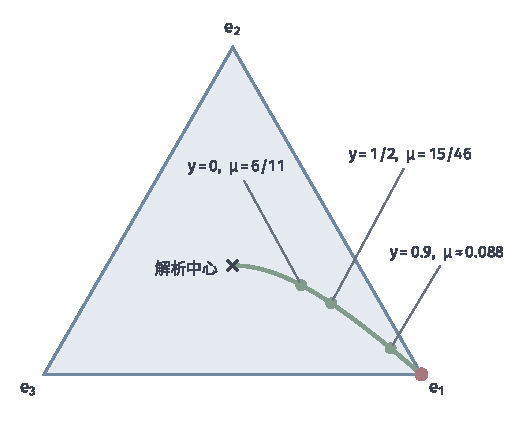
\includegraphics[width=90mm]{figures/05-optimization/01-linear-programming/matplotlib/lpipm-central-path/figure.pdf}
  \caption{贯穿例的中心路径。三角形是可行集，三个角是单位向量，黑叉是解析中心$(1/3,1/3,1/3)^\top$，绿线是中心路径，绿点是例~\ref{ex:lpipm-central-closed-form}算出的中心点以及$y=0.9$的中心点，红点是最优顶点$\bm{e}_1$。}
  \label{fig:lpipm-central-path}
\end{BookInlineFigure}

\paragraph{间隙恰好是$n\mu$}
中心路径最有用的性质是，沿路径的对偶间隙可以直接读出来。中心点原始、对偶都可行，把式~\eqref{eq:lpipm-gap-identity}用到这里，再代入$x_is_i=\mu$，得到
\begin{equation}
 \bm{c}^\top\bm{x}(\mu)-\bm{b}^\top\bm{y}(\mu)=\sum_{i=1}^nx_i(\mu)s_i(\mu)=n\mu.
 \label{eq:lpipm-central-gap}
\end{equation}

它把“还差多远”变成了一个已知的数。由弱对偶$\bm{b}^\top\bm{y}(\mu)\leq p^\star$，原始目标误差不超过间隙：
\begin{equation}
 \bm{c}^\top\bm{x}(\mu)-p^\star\leq n\mu.
 \label{eq:lpipm-central-error}
\end{equation}
要让误差不超过$\varepsilon$，走到$\mu\leq\varepsilon/n$就够了。在例~\ref{ex:lpipm-central-closed-form}中，$y=0$的中心点目标值是$6/11+6/11+6/11=18/11$，对偶目标是$0$，间隙$18/11$正好等于$3\mu$。

这个结论用到了精确的中心点。迭代算法只能走到中心路径附近，这时间隙怎样计算，第~\ref{sec:lpipm-accuracy}节会逐项说明。

\paragraph{路径的终点}
式~\eqref{eq:lpipm-central-gap}说明目标值收敛到最优值，却没有说点本身收敛到哪里。解不唯一时，这个问题的答案并不平凡。先看例子：把目标换成$c=(0,0,1)$，约束不变，此时第三个分量为零的整条边都是最优解。

这时$\bm{s}=(-y,-y,1-y)$，记$r=-y>0$，则$x_1=x_2=\mu/r$，$x_3=\mu/(1+r)$，等式约束给出
\[
 \frac{2\mu}{r}+\frac{\mu}{1+r}=1.
\]
令$\mu\downarrow0$，第二项趋于零，第一项必须趋于$1$，所以$r\approx2\mu$，$x_1=x_2=\mu/r\to1/2$。路径的极限是$(1/2,1/2,0)^\top$，它不是顶点，而是最优边的中点，如图~\ref{fig:lpipm-optimal-face}(b)所示。

\begin{BookInlineFigure}
  \centering
  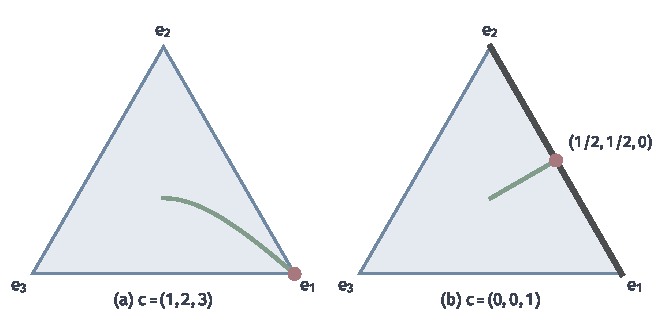
\includegraphics[width=112mm]{figures/05-optimization/01-linear-programming/matplotlib/lpipm-optimal-face/figure.pdf}
  \caption{路径的极限由最优解集决定。绿线是中心路径。(a)$\bm{c}=(1,2,3)$，最优解唯一，路径通向顶点$\bm{e}_1$（红点）。(b)$\bm{c}=(0,0,1)$，最优解集是深灰粗线表示的整条边，路径通向这条边的中点$(1/2,1/2,0)^\top$，这是最优面上的解析中心，不是顶点。}
  \label{fig:lpipm-optimal-face}
\end{BookInlineFigure}

一般情形的结论如下。设最优解集合为$\bm{S}_{\mathrm{P}}$，这是可行集的一个面，称为\term{最优面}（optimal face）。若某对原始、对偶最优解满足对每个下标$x_i^\star+s_i^\star>0$，就称这对解是\term{严格互补}（strictly complementary）的。下面的定理说，中心路径收敛到一对严格互补的解，并且在最优面上取在“最中央”的位置。

\begin{theorem}[中心路径的极限]
\label{thm:lpipm-central-limit}
设$\bm{A}$满行秩，$\mathcal{F}^{\circ}$非空。当$\mu\downarrow0$时，$(\bm{x}(\mu),\bm{y}(\mu),\bm{s}(\mu))$收敛到一对最优解$(\hat{\bm{x}},\hat{\bm{y}},\hat{\bm{s}})$。记$B=\{i:\hat{x}_i>0\}$，$N=\{i:\hat{s}_i>0\}$，则$B$与$N$互不相交且并集为$\{1,\ldots,n\}$，并且$\hat{\bm{x}}$是最优面上使下式最大的唯一点：
\begin{equation}
 \sum_{i\in B}\log x_i.
 \label{eq:lpipm-face-center}
\end{equation}
\end{theorem}

\begin{proof}
关键工具是一个正交关系。设$\bm{x},\bm{x}'$都满足等式$\bm{A}\bm{x}=\bm{b}$，$(\bm{y},\bm{s}),(\bm{y}',\bm{s}')$都满足$\bm{A}^\top\bm{y}+\bm{s}=\bm{c}$。则$\bm{x}-\bm{x}'$属于$\bm{A}$的零空间，$\bm{s}-\bm{s}'=-\bm{A}^\top(\bm{y}-\bm{y}')$属于$\bm{A}^\top$的列空间，于是
\begin{equation}
 (\bm{x}-\bm{x}')^\top(\bm{s}-\bm{s}')=0.
 \label{eq:lpipm-orthogonality}
\end{equation}

\emph{有界性。}取固定的$(\bar{\bm{x}},\bar{\bm{y}},\bar{\bm{s}})\in\mathcal{F}^{\circ}$。把式~\eqref{eq:lpipm-orthogonality}用到中心点和这一点，展开并用$\bm{x}(\mu)^\top\bm{s}(\mu)=n\mu$，得到
\[
 \bar{\bm{s}}^\top\bm{x}(\mu)+\bar{\bm{x}}^\top\bm{s}(\mu)=n\mu+\bar{\bm{x}}^\top\bar{\bm{s}}.
\]
左边各项非负且$\bar{\bm{x}},\bar{\bm{s}}>\bm{0}$，所以$\mu\in(0,1]$时$\bm{x}(\mu)$、$\bm{s}(\mu)$有界。$\bm{A}^\top$列满秩，$\bm{y}(\mu)$也有界。

\emph{聚点是最优解。}取$\mu_k\downarrow0$使三元组收敛到一个聚点$(\hat{\bm{x}},\hat{\bm{y}},\hat{\bm{s}})$。它满足两组等式，$\hat{\bm{x}},\hat{\bm{s}}\geq\bm{0}$，且由式~\eqref{eq:lpipm-central-gap}，$\hat{\bm{x}}^\top\hat{\bm{s}}=0$，所以是最优解。

\emph{一个归一化的恒等式。}设$(\bm{x}^\star,\bm{y}^\star,\bm{s}^\star)$是任意一对最优解，由互补松弛，它们的内积为零。把式~\eqref{eq:lpipm-orthogonality}用到中心点和这一对最优解，得到
\[
 (\bm{s}^\star)^\top\bm{x}(\mu)+(\bm{x}^\star)^\top\bm{s}(\mu)=n\mu.
\]
两边除以$\mu$，用$x_i(\mu)/\mu=1/s_i(\mu)$和$s_i(\mu)/\mu=1/x_i(\mu)$，得到
\begin{equation}
 \sum_{i=1}^n\frac{s_i^\star}{s_i(\mu)}+\sum_{i=1}^n\frac{x_i^\star}{x_i(\mu)}=n.
 \label{eq:lpipm-normalized}
\end{equation}

\emph{严格互补。}式~\eqref{eq:lpipm-normalized}左边每一项非负，所以$x_i(\mu)\geq x_i^\star/n$。令$\mu=\mu_k\to0$，得$\hat{x}_i\geq x_i^\star/n$，即每个最优解的正分量也是$\hat{\bm{x}}$的正分量；对$\hat{\bm{s}}$同理。

再把聚点$(\hat{\bm{x}},\hat{\bm{s}})$本身当作最优解代入式~\eqref{eq:lpipm-normalized}，令$\mu_k\to0$。$i\in B$时$\hat{x}_i/x_i(\mu_k)\to1$，$i\in N$时$\hat{s}_i/s_i(\mu_k)\to1$，其余项为零，于是
\[
 \lvert B\rvert+\lvert N\rvert=n.
\]
互补性$\hat{\bm{x}}^\top\hat{\bm{s}}=0$说明$B\cap N=\varnothing$，所以它们的并集是全部下标。

\emph{极限唯一。}由上一步，任何聚点的正分量位置都包含任何最优解的正分量位置，所以所有聚点有相同的$B$和$N$，任何原始最优解在$N$上为零。在式~\eqref{eq:lpipm-normalized}中取$\bm{s}^\star=\hat{\bm{s}}$、$\bm{x}^\star$为任意原始最优解，令$\mu_k\to0$，得到
\[
 \lvert N\rvert+\sum_{i\in B}\frac{x_i^\star}{\hat{x}_i}=n,\qquad\text{即}\qquad\sum_{i\in B}\frac{x_i^\star-\hat{x}_i}{\hat{x}_i}=0.
\]
这正是凹函数~\eqref{eq:lpipm-face-center}在$\hat{\bm{x}}$处沿任意最优面方向的方向导数为零，所以$\hat{\bm{x}}$是它在最优面上的最大点。严格凹性保证最大点唯一，因此所有聚点的$\bm{x}$部分相同。对$\hat{\bm{s}}$同理，得到相应的$\sum_{i\in N}\log s_i$最大的唯一点，再由$\bm{A}^\top$列满秩，$\hat{\bm{y}}$也唯一。有界序列只有一个聚点，所以收敛。
\end{proof}

这个定理有两个直接的推论。最优解唯一时，路径通向顶点；最优解不唯一时，路径通向最优面的相对内部，得不到顶点。此外，定理顺带证明了线性规划在$\mathcal{F}^{\circ}$非空时总有严格互补解。

这里的下标集$B$和单纯形法的基不是一回事：$B$是极限点的正分量位置，可以多于或少于$m$个。内点法最终告诉我们的是“哪些变量为正”，而不是直接给出一个基，第~\ref{sec:lpipm-accuracy}节会处理两者的转换。
